%!TEX root = ../memoire.tex

\chapter{GenDR}\label{chapgendr}

GenDR (Generic Deep Realizer) est un réalisateur profond multilingue \citep{lareau18}. Il a hérité de l'architecture de MARQUIS. C'est-à-dire que GenDR modélise le langage dans des paramètres similaires, utilise le même transducteur de graphe et se sert de la même théorie linguistique. GenDR se démarque par sa capacité à traiter des phénomènes langagiers complexes en traitant l'interface sémantique-syntaxe en profondeur. Il offre une couverture beaucoup plus importante que MARQUIS en ce qui concerne les locutions, les collocations via un traitement large des fonctions lexicales. Cette couverture lexicale a été opérée par Lareau et Lambrey \cite{LambreyImplementationcollocationspour2017}, \cite{lambrey15}. Mais couvre la réalisation jusqu'à la syntaxe de surface, ne se rend pas jusqu'au bout.

Tel que mentionné, GenDR est une grammaire multilingue. Les règles grammaticales de base sont directement héritée de MARQUIS(citation) qui pouvait réaliser du texte en : catalan, anglais, français, polonais, portugais et espagnol. Ils n'ont gardé que les règles de base qui décrivent des phénomènes langagiers de base: lexicalisation simple, complementation, modification,etc. Ces règles forment le noyau du système et sont partagées (la majorité) par l'ensemble des langues du systèmes. Les règles spécifiques aux langues modélisent des phénomènes comme la sélection des auxiliaires, les déterminants, etc.

Le mapping entre les graphes sémantiques et les structures syntaxiques de surface se fait en deux étapes. Ces deux étapes sont effectuées par l'entremise de deux modules de règles différents opérant les interfaces respectives. Le module sémantique mappe les graphes sémantiques aux structures syntaxiques profondes correspondantes (Melcuk,2013), tandis que le module syntaxique mappe les structures syntaxiques profondes aux strucutres syntaxiques de surface. Cette architecture stratifiée est directement inspirée de la théorie Sens-Texte (melcuk et compagnie).

Ainsi le module sémantique contient 21 règles dont la plupart sont héritées de MARQUIS et 132 règles de lexicalisation \citep{LambreyImplementationcollocationspour2017}. Pour sa part, le module syntaxique contient nettement moins de règles. 20 règles dont 12 partagées entre les langues. Chaque règle modélise un phénomène langagier sur quoi la grammaire compte sur la richesse des dictionnaires.

%%%%%%%%%%%%%%%%%%%%%%%%%%%%%%%%%%%%%%%%%%%%%%%%%%%%%%%
% --------- A R C H I T E C T U R E  GENDR  ---
%%%%%%%%%%%%%%%%%%%%%%%%%%%%%%%%%%%%%%%%%%%%%%%%%%%%%%%
\section{Architecture de GenDR}

Dans la section suivante, nous allons brièvement présenter MATE, la plateforme sur laquelle GenDR fonctionne. Nous allons ensuite brièvement décrire la composante multilingue de GenDR.

\subsection{MATE}
\citep{Lareau2007TowardsAG}

MATE a été créé par Bernd Bohnet. Sa raison d'être provient du désir d'implémenter les couches de représentations à la Théorie Sens-Texte dans un transducteur de graphe. Ainsi, la transduction d'un graphe à un autre correspond au passage d'une couche de représentation à une autre. Ce logiciel permet aussi de tester, développer et maintenir la tâche qu'est la réalisation linguistique dans le cadre de la \ac{GAT} citep{BohnetDevelopmentEnvironmentMTTbased2000}. Afin de développer et tester le matériel, MATE comprend les composantes suivantes : un éditeur de dictionnaire, de graphes et de grammaires. Les dictionnaires encodent les unités sémantiques, lexicales et fonctionnelles. Les grammaires sont composées de règles modélisant le passage d'une représentation à une autre. C'est via les règles que la transduction de graphes se fait. L'éditeur de graphes permet de construire l'input et de le visualiser soit en format textuel ou graphique. Il y aussi un module d'inspecteur permettant de voir le déroulement de l'application des règles. Autrement dit, chaque étape de la transduction est explicitée et cela nous permet de voir quelles règles ont été utilisées ou quelles règles auraient dû être utilisées. Pour plus de détails concernant ce système, nous vous référons à ces articles \citep{BohnetDevelopmentEnvironmentMTTbased2000}, \citep{BohnetOpensourcegraph2010},\citep{LambreyImplementationcollocationspour2017}.

Nous allons maintenant montrer brièvement à quoi ressemble les éditeurs dictionnairiques, grammaticaux et graphiques.
%%%%%%%%%%%%%%%%%%%%%%%%%%%%%%%%%%%%%%%%%%%%%%%%%%%%%%%
% ---------D I C T I O N N A I R E  ------------------
%%%%%%%%%%%%%%%%%%%%%%%%%%%%%%%%%%%%%%%%%%%%%%%%%%%%%%%

\subsubsection{Dictionnaires}\label{dictio}
GenDR se sert de trois dictionnaires: un dictionnaire sémantique, un dictionnaire lexical et un dictionnaire de fonctions lexicales. Puisque les fonctions lexicales en génération automatique de texte ont déjà traitées par \cite{LambreyImplementationcollocationspour2017}, nous ne n'élaborerons pas sur ce dictionnaire. D'abord, le dictionnaire sémantique sert à encoder les unités sémantiques qui composent les noeuds des graphes d'entrées. Voici un entrée typique dans un dictionnaire sémantique (\emph{semanticon})

\begin{lstlisting}[language=Xml, caption = semanticon, label = semanticon]
owe { lex = owe
      lex = debt }
\end{lstlisting}
Ce dictionnaire mappe les sémantèmes à des lexèmes ou des locutions. Un même sémantème peut ainsi pointer vers deux lexèmes synonymes, mais aussi vers deux lexèmes signifiant la même chose, mais appartenant à des parties du discours différentes. Par exemple owe(sens) correspond à owe(lexème) un verbe, et debt(lexème) un nom.

Le dictionnaire lexical contient ce genre d'information:
\begin{lstlisting}[language=Xml, caption = lexicon]
verb_dit : verb_dt {                   // direct transitive
  gp = {
     III = {
        dpos = N
        rel = indir_objective
        prep = to  

     }
  }
}
[...]
owe : verb_dit {
  gp = { II = { dpos=Num } }
  gp = { II = { dpos=N } }
}
\end{lstlisting}
information détaillée à propos de chaque unité lexicale d'une langue. Les lexèmes et locutions ont leurs entrée dans ce dictionnaire. Une entrée a : PDD, diathèse, sous-catégorisation et collocations contrôlées. MATE incorpore aussi des mécanismes d'héritage facilitant l'encodage des ressources lexicales. Il est possible de créer des classes, et lorsqu'on pointe une unité vers une classe, elle hérite de tous les traits de cette classe. C'est de cette manière qu'on peut créer des classes de verbes. Par exemples, owe est un verbe ditransitif et il pointe vers la classe de verbe ditransitif. Cette classe a des traits X, mais elle hérite des traits de la classe verb transitif qui contient les traits communs à tous les verbes direct, puis cette classe hérite de verb qui contient les traits communs à tous les verbes. 

1500 mots les plus courants de fr et ang, puis quelques persan et lithuanien.

%%%%%%%%%%%%%%%%%%%%%%%%%%%%%%%%%%%%%%%%%%%%%%%%%%%%%%%
% ---------G R A M M A I R E  ------------------
%%%%%%%%%%%%%%%%%%%%%%%%%%%%%%%%%%%%%%%%%%%%%%%%%%%%%%%

\subsubsection{Grammaires}

\begin{figure}[htb]
	\centering
	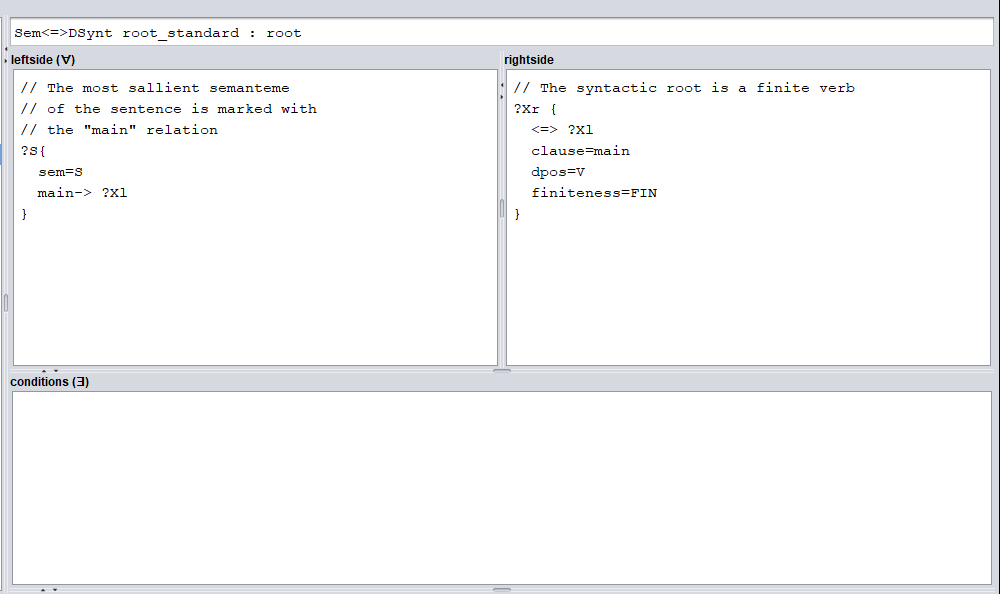
\includegraphics[width=1\textwidth, trim = {0cm 0cm 0cm 0cm},clip]{ch3/figs/grammaire.png}
	\caption{Règle créant la racine syntaxique}
	\label{fig:root}
\end{figure}

Donc, en haut, on a : interface, nom de la règle et regroupement de règles. Le côté leftside est le point de départ de la transduction. Le côté droit est l'arrivée de la transduction. La partie en bas est les conditions. C'est là qu'on encode toutes les règles et dans ce format. Nous reviendrons aux règles dans la section exemple

%%%%%%%%%%%%%%%%%%%%%%%%%%%%%%%%%%%%%%%%%%%%%%%%
% ---------G R A P H E S ------------------
%%%%%%%%%%%%%%%%%%%%%%%%%%%%%%%%%%%%%%%%%%%%%%%%

\subsubsection{Graphes}\label{entree-sortie}
\draft{mettre les labels des figures au lieu de dire: figure suivante}
L'input de GenDR est un graphe sémantique de type TST. Dans celui-ci les prédicats sont liés à leurs arguments par des relations étiquettées avec des chiffres indiquant la position de l'argument. L'une des unités sémantiques doit être identifiée comme étant la plus saillante de l'énoncé. Il s'agit du noeud dominant de la phrase. Lors du transfert à la syntaxe profonde, il sera mappé comme racine syntaxique (le sommet de l'arbre).

Voici à quoi ressemble l'input :
\begin{lstlisting}[language=XML, caption = Input sémantique, label=input]
structure Sem debt {
S {
owe {
tense=PRES
1-> Paul {class=proper_noun}
2-> "\$500K" {class=amount}
3-> bank {number=SG definiteness=DEF}}
main-> owe}}
\end{lstlisting}

Mais pour simplifier la chose, nous montrerons une version graphique
\begin{figure}[htb]
	\centering
	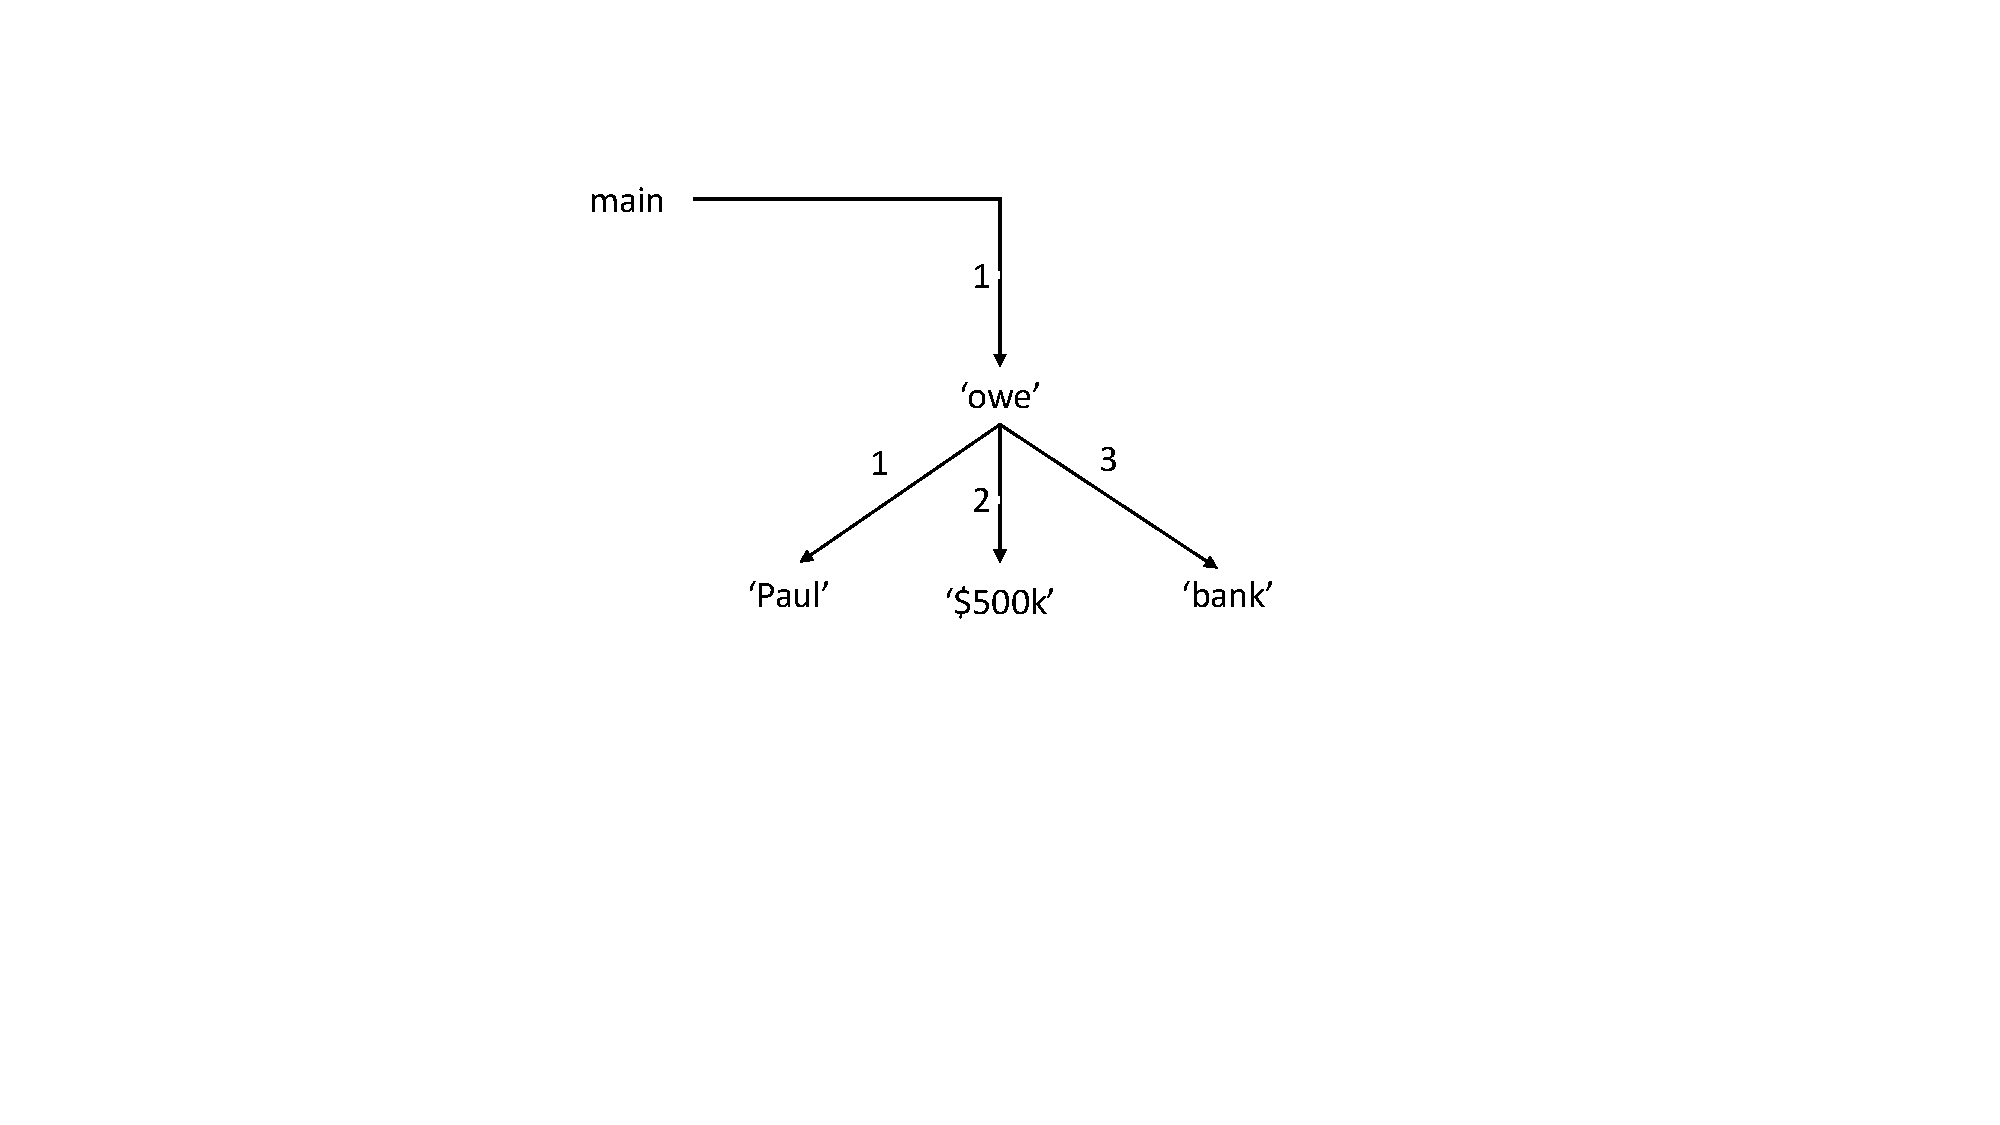
\includegraphics[width=1\textwidth, trim = {0cm 4cm 0cm 3cm},clip]{ch3/figs/owe_sem.pdf}
	\caption{Graphe sémantique en visuel}
	\label{fig:graphesem}
\end{figure}

L'output de ce système consiste en un ensemble de structures de dépendances syntaxiques de surface. Ainsi, avec l'input sémantique en \ref{input} le réalisateur génère les six structures suivantes. Effectivement, c'est la preuve de la flexibilité du réalisateur GenDR. 

\begin{figure}[htb]
	\centering
	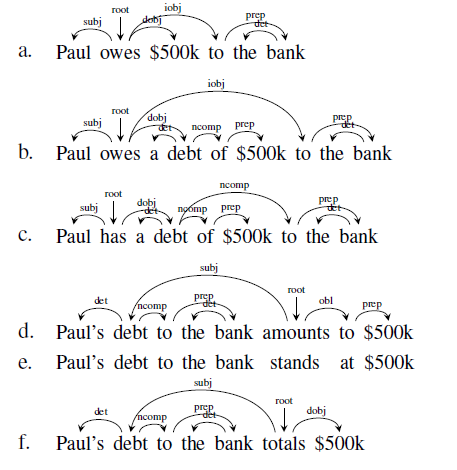
\includegraphics[width=0.5\textwidth, trim = {0cm 0cm 0cm 0cm},clip]{ch3/figs/exemples_real.png}
	\caption{6 réalisations syntaxe de surface}
	\label{fig:realsurf}
\end{figure}

Toutefois, dans cette figure, les arbres de dépendances ont été linéarisés pour faciliter la compréhension du lecteur. Dans les faits, les arbres générés en output ne sont pas linéarisés. Il s'agit toujours d'arbres de dépendances en syntaxe de surface. 

\begin{figure}[htb]
	\centering
	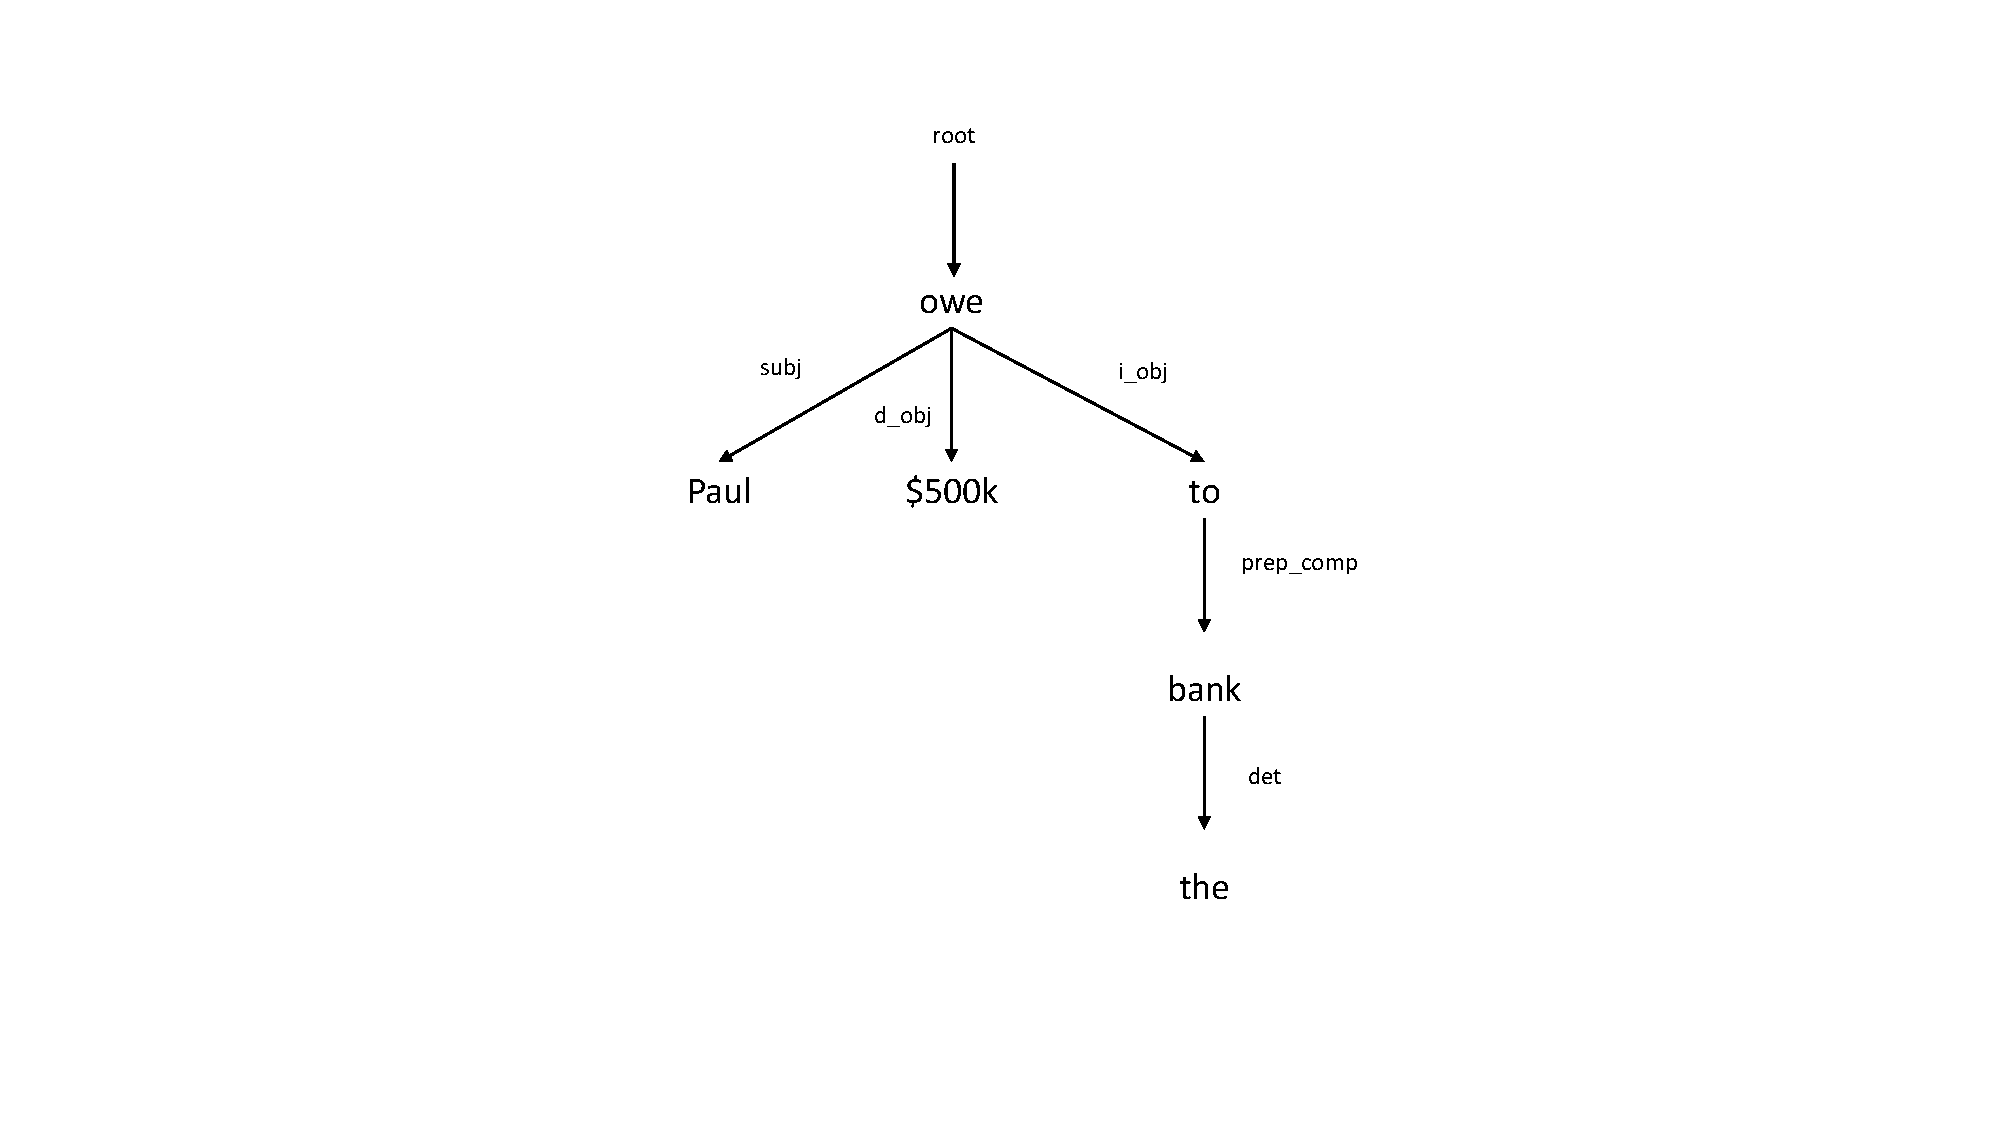
\includegraphics[width=1\textwidth, trim = {0cm 2cm 0cm 2cm},clip]{ch3/figs/realsurfex.pdf}
	\caption{Réalisation de surface}
	\label{fig:realsurfex}
\end{figure}

Si on souhaite une réalisation linéarisée,  il faudra passer par un réalisateur de surface. GenDR ne traite pas l'interface morpho-syntaxique et ne linéarise pas le texte. C'est dans ces contextes, que les réalisateurs de surface mentionnées précédement entrent en jeu. Les forces de GenDR concernent les tâches plus profondes de la réalisation, notamment l'arborisation et la lexicalisation.

%%%%%%%%%%%%%%%%%%%%%%%%%%%%%%%%%%%%%%%%%%%%%%%%%%%%%%%%%%%%%%%%%%%%%%%%%%%%%
% --------- I N T E R F A C E   S É M A N T I Q U E- S Y N T A X E ---------
%%%%%%%%%%%%%%%%%%%%%%%%%%%%%%%%%%%%%%%%%%%%%%%%%%%%%%%%%%%%%%%%%%%%%%%%%%%%%

\section{Interface sémantique-syntaxe en TST}

Ainsi, tel que mentionné, nous utilisons des graphes sémantiques en entrée dans ce système. Pour mieux comprendre de quoi il s'agit, nous ferons un retour sur les fondements de la théorie Sens-Texte

Pourquoi la TST : importante dans le domaine{Vicentegeneracionlenguajenatural2015} et a fait ses preuves avec MARQUIS, FORGe, RealPro.

Expliquer en quoi l'interface sémantique-syntaxe permet de réaliser des phénomènes linguistiques plus profonds que les réalisateurs de surface (peut-être faire un petit retour sur ce qui a été dit). Cette interface implique deux processus intimement liés : l'arborisation et la lexicalisation. 

%%%%%%%%%%%%%%%%%%%%%%%%%%%%%%%%%%%%%%%%%%%%
% ---------T H É O R I Q U E  ------
%%%%%%%%%%%%%%%%%%%%%%%%%%%%%%%%%%%%%%%%%%%

\subsection{Arborisation théorique}\label{arbo}
Pour mieux comprendre ce qu'est l'arborisation, nous ferons un court retour sur la Théorie Sens-Texte. C'est une théorie linguistique qui vise la description de la correspondance entre le Sens et le Texte (comme son nom l'indique). Celle-ci se fait via la construction de modèles formels \citep{PolgueretheorieSensTexte1998}. Le schéma \ref{fig:modeletst} présente comment on schématise le fonctionnement de ces modèles.

\begin{figure}[htb]
	\centering
	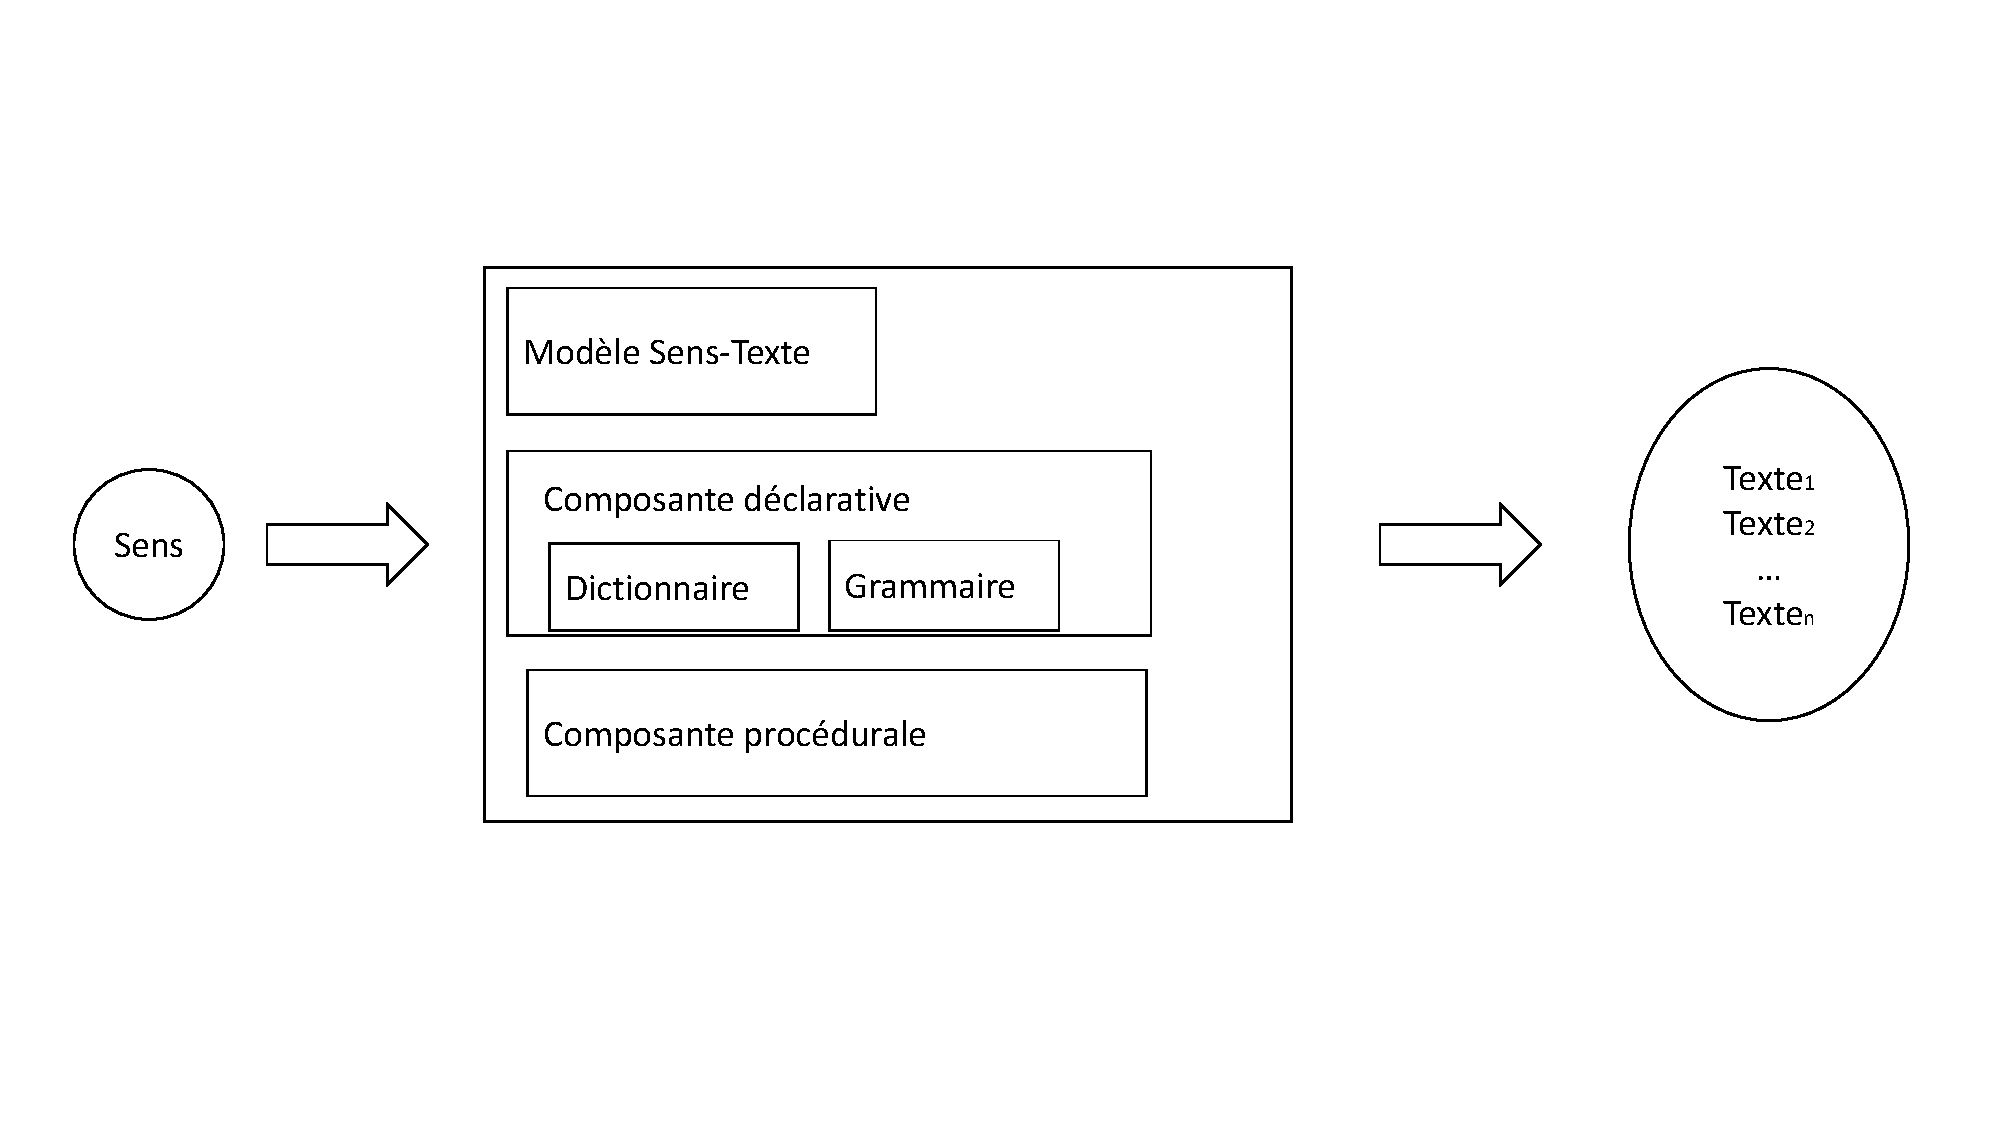
\includegraphics[width=1\textwidth, trim = {0cm 3cm 0cm 3cm},clip]{ch3/figs/polguere1.pdf}
	\caption{Structure d'un modèle TST}
	\label{fig:modeletst}
\end{figure}

La figure \ref{fig:modeletst} provient de Polguere 1998. illustre le fait qu'un modèle Sens-Texte est une machine virtuelle qui prend en entrée des représentations de sens d'énoncés et retourne en sortie un ensemble de Textes, qui contient toutes les paraphrases permettant d'exprimer le Sens donné en entrée. 

Tel qu'on l'a vu dans l'exemple en \ref{entree-sortie}. Ainsi, pour ce rendre au format de sortie, la représentation sémantique a subie diverses opérations qui lui ont permis de traverser divers niveaux de représentations. Pour illustrer ces représentations, nous vous renvoyons au tableau \ref{fig:processustst}.

\begin{figure}[htb]
	\centering
	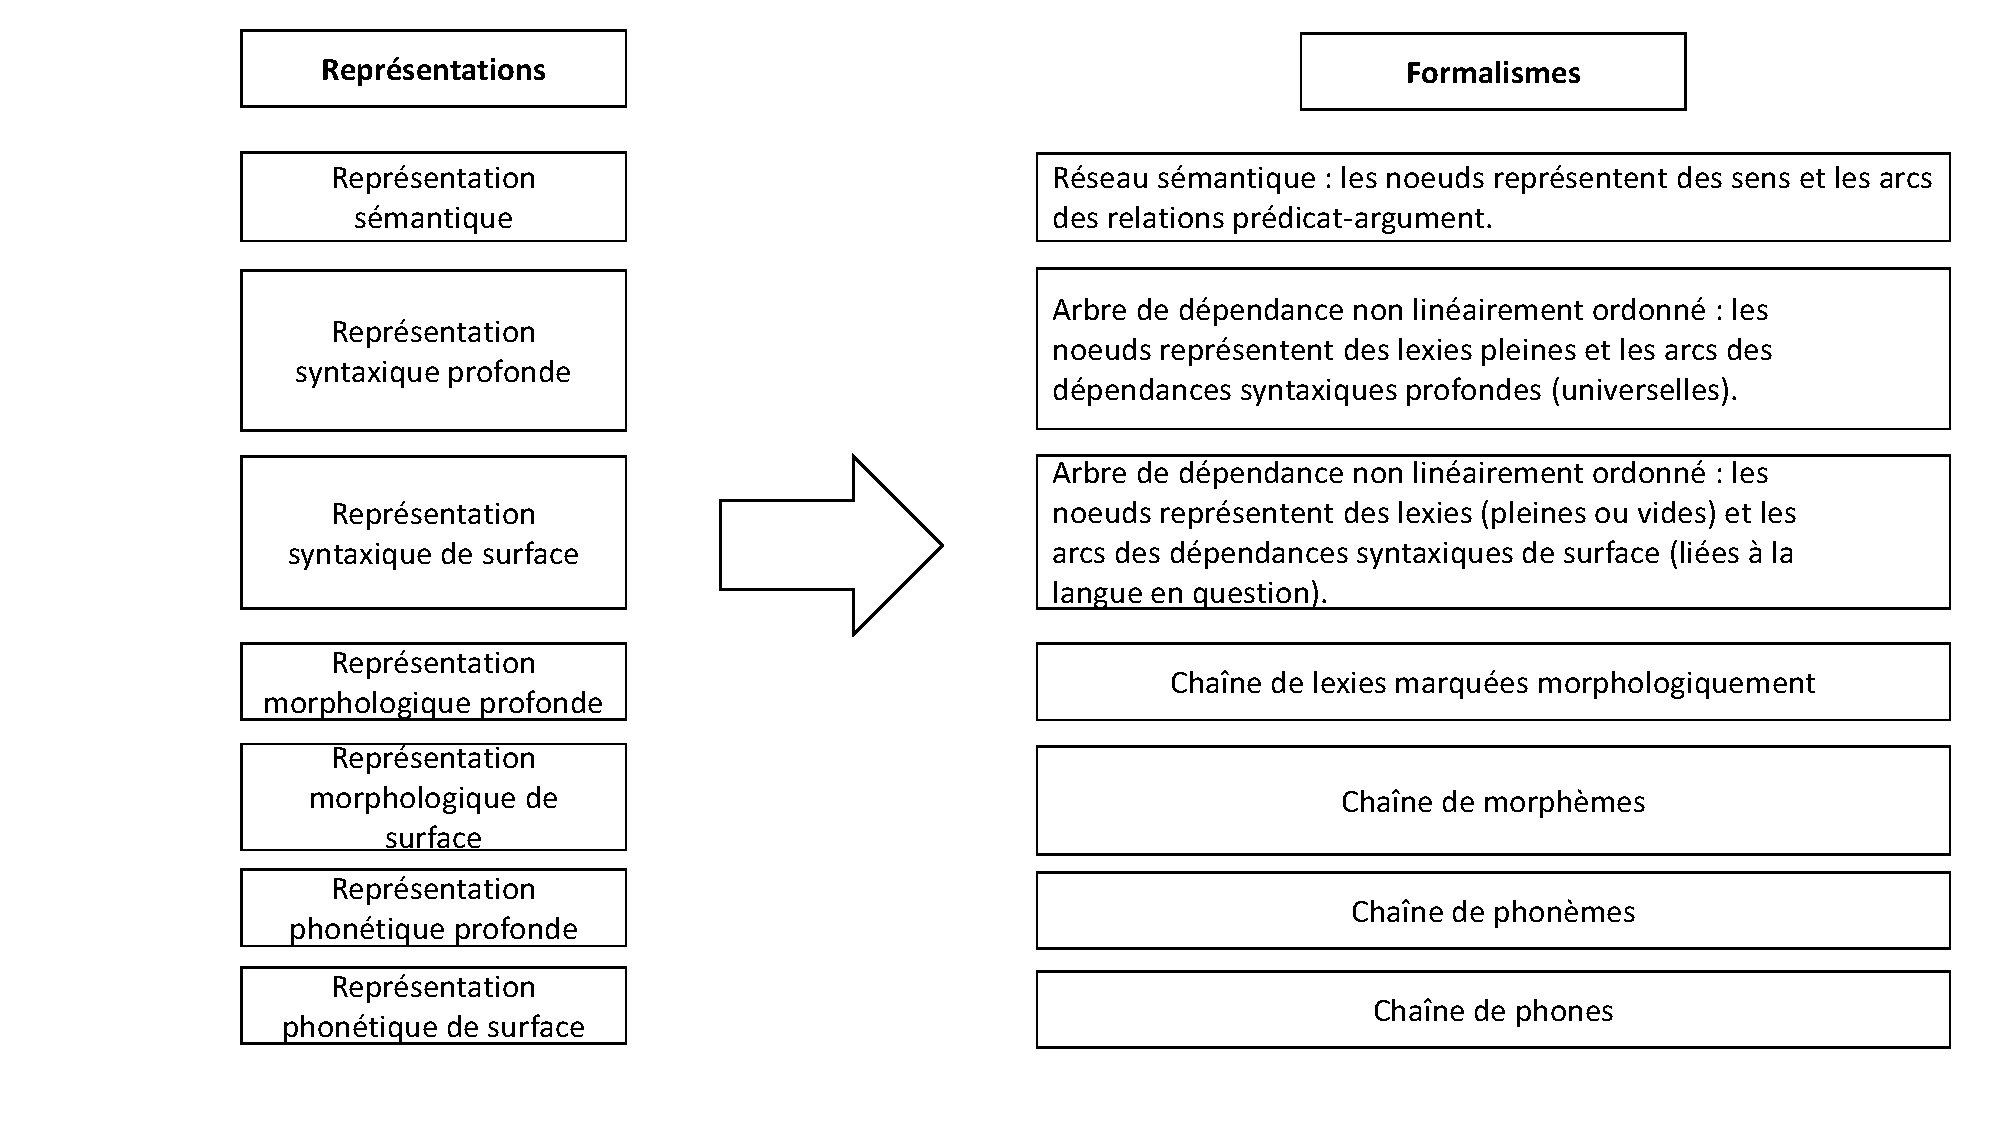
\includegraphics[width=1\textwidth, trim = {0cm 0cm 0cm 0cm},clip]{ch3/figs/polguere2.pdf}
	\caption{Processus d'un modèle TST}
	\label{fig:processustst}
\end{figure}

Dans le cadre de ce travail, nous ne nous intérresserons qu'aux niveaux de rep sémantique jusqu'à syntaxe de surface. Car, comme nous l'avons mentionné précédemment, GenDR est un réalisateur profond qui opère uniquement dans ces niveaux de représentations. C'est pourquoi nous allons expliquer plus en détails de le transfert d'information entre ces niveaux de représentations et les modules linguistiques requis pour passer de RSem à RSyntP, puis à RSyntS.

Selon la TST, la structure syntaxique d'un énoncé représente l'ensemble des liens de dependance fonctionnelle qui existe entre les unités lexicales de cet énoncé. On représente formellement ces structures syntaxiques par des arbres qui sont caractérisés comme des arbres de dépendances. Cette approche syntaxique provient de Tesnière 1965. Bref, comme on l'a montré dans le schéma en \ref{fig:processustst}, il y existe deux niveaux de représentation syntaxique en TST : la RSyntP et la RSyntS. Pour mieux les comprendre nous les décrirons. D'abord, la RSyntP prend son origine dans la RSem. Ainsi, les relations et les lexies qui existent en RSyntP sont des conséquences directes d'une transition de la RSem. Formellement, le passage de la RSem à la RSyntP se nomme l'arborisation. Car on cherche à arboriser la RSem et cela donne en conséquence un arbre de dépendance en RSyntP.Ce passage est effectuée via des règles de correspondance sémantiques. Ces règles sont la partie 'grammaire' du schéma montré plutôt à la figure \ref{fig:modeletst}.

Pour que l'arborisation se fasse correctement, la première étape est d'identifier l'unité sémantique qui correspondera à la racine de l'arbre syntaxique profond. Une fois que nous avons cette racine (la hiérarchisation) \citep{PolguereStructurationmisejeu1990}. Cette hiérarchisation est aussi prise en compte par le système de règles de correspondances sémantiques. Une fois que cette étape est fait, on va partir de ce noeud en sémantique pour lexicaliser les noeuds qui lui sont liés et par le fait même réaliser les règles actancielles qui permettent la transition de la sémantique à la syntaxe des relations prédicats-arguments. citation"chaque arc est considéré successivement dans l'ordre du parcours, puis est traduit en une micro-structure syntaxique profonde grâce aux règles de correspondance sémantique de la grammaire." p.273 de \citep{PolguereStructurationmisejeu1990}. 


\draft{- construire le sommet de l'arbre syntaxique profond, qui correspond au ND de la RSémR
- construire récursivement toutes les relations actancielles syntaxiques dépendant du sommet de l'arbre.}

Une fois que l'arborisation est complétée, l'arbre de dépendance profond transitera vers un niveau de surface. Cette transition implique les opérations suivantes. D'abord, faire le calcul des relations syntaxiques de surface. Ainsi, la relation I deviendra sujet, la relation II deviendra complément d'objet direct, etc. Pour une meilleure compréhension, nous ferons un exemple plus bas. On incorpore à ce stade les lexies vides (prépositions, déterminants, etc.). La pronominalisation fait aussi partie de cette étape. Ainsi que la construction des structures communicative, anaphorique et prosodique du niveau syntaxique de surface. Mais, ces deux étapes ne sont pas effectuée dans GenDR.

\subsection{lexicalisation théorique}

La lexicalisation se passe entre le niveau RSem et la RSyntP \citep{PolguereStructurationmisejeu1990}. Le but est de choisir les unités sémantiques qui seront réalisées en syntaxe profonde en tant que lexèmes (unité lexicale). La lexicalisation est ainsi très liée à l'arborisation car ce sont deux étapes qui se produisent lors du passage de la RSem à la RSyntP. D'ailleurs, ces deux étapes se produisent simultanément. Effectivement la construction de la représentation syntaxique profonde est une conséquence de l'arborisation des liens de la représentation sémantique et de la lexicalisation des unités sémantiques. Ce qui résulte en un arbre de dépendance lexicalisé.

%%%%%%%%%%%%%%%%%%%%%%%%%%%%%%%%%%%%%%%%%%%%%%%%%%%%%
% --------- C O M P U T A T I O N N E L L E  ------
%%%%%%%%%%%%%%%%%%%%%%%%%%%%%%%%%%%%%%%%%%%%%%%%%%%%

\section{Arborisation et lexicalisation computationnelle}

Maintenant que nous avons présenté le côté théorique de l'interface sémantique-syntaxe, nous exposerons comment ces mécanismes se transposent dans GenDR.

\subsection{Arborisation computationnelle}
Tel que mentionné à la \draft{section \ref{arbo}}, on identifiait un noeud dans la structure d'input comme étant le noeud principal. Il faut faire cela car un graphe sémantique n'a naturellement pas de point d'ancrage. Or, si on veut générer une structure où l'un des sens est le noeud principal, il faut l'indiquer dans la structure d'input. Par exemple, si on voulait réaliser l'input sémantique suivant sans préciser le noeud principal \draft{reprendre l'exemple de françois}. On peut ainsi laisser le soin à GenDR de choisir le noeud principal, mais en règle général, on veut contrôler la structure communicative de l'output. L'arbre syntaxique profond est construit avec un algorithme top-down. Le top étant le noeud identifié comme noeud principal. L'arbre syntaxique est ainsi construit en se basant sur le graphe sémantique. L'algo est ressemble beaucoup à celui de MARQUIS et FORGe puisqu'ils sont tous des tenants de la TST. 

L'arborisation dans GenDR se fait en trois étapes. Nous les décrirons à la section suivante.

\subsubsection{Règles de base pour l'arborisation}

1.root\_standard On construit la racine de l'arbre syntaxique et on la fait correspondre au noeud principal de la structure sémantique. À cette étape, on crée seulement le noeud sans le lexicaliser. Mais on lui ajoute des contraintes. La contrainte principale est qu'il doit s'agir d'un verbe avec le mood indicatif (bien que des règles autres pourraient produire contrôler des alternatives). Cette étape n'arrive qu'une fois par graphe, par après, on ne se sert plus de celle-ci.

2. Une fois que le noeud a été créé et contraint en syntaxe profonde, on cherche dans notre grammaire pour une règle de lexicalisation qui peut satisfaire les contraintes, puis on regarde dans le dictionnaire pour un lexème qui correspond au sens demandé et aux contraintes demandées.

3.actant\_gp, actant\_guess, attr\_lex. 
Une fois que le noeud racine a été lexicalisée dans la structure syntaxique profonde, on regarde les arcs en relation avec le noeud sémantique principal. Donc on retourne voir dans le graphe sémantique. Les arcs qui partent du noeud sémantique pointant vers ses arguments sont réalisés comme des compléments. Tandis que les arcs qui pointent vers le noeud seront réalisés comme des modificateurs. En syntaxe profonde cette relation sera réalisée comme un dépendant du noeud étiquetté ATTR. Si l'argument réalisé est un complément, on doit regarder dans le patron de régime du gouverneur dans le dictionnaire. Le GP donne de l'information à propos du mapping sémantique, syntaxique profond, syntaxique surface des actants d'un lexème. Le GP spécifie aussi la partie du discours des compléments sélectionnés et les prépositions si nécessaires. Cette étape crée de nouveaux noeuds, mais pas lexicalisés, mais qui ont des contraintes. Pour chacun de ces noeuds, on retourne à l'étape 2, puis cycliquement, nous retournons à l'étape 3,  jusqu'à ce que le graphe sémantique soit complètement réalisé en surface profonde.

\subsection{Lexicalisation computationnelle}

La lexicalisation dans GenDR implique trois niveaux de représentations : la sémantique, syntaxe profonde, syntaxe de surface. La première étape est de prendre une unité lexicale profonde servant à exprimer un sémantème donné. Ça c'est la lexicalisation profonde. Elle introduit des mots pleins de sens et des verbes supports. Puis les lexèmes de surface sont choisis pour exprimer les unités lexicales profondes. Il s'agit de la lexicalisation superficielle. Celle-ci introduit les mots fonctions.

GenDR performe 6 types de lexicalisation. Celles-ci sont produites par l'intéraction des règles et des dictionnaires : lexicalisation simple pour les lexèmes, lexicalisation de patron pour les idiômes, bound lexicalisation pour les collocations, lexicalisation à base de classes pour les noms propres,etc. et lexicalisation fallback pour les mots inconnus et lexicalisation grammaticale pour les mots fonctions.  Nous ne traiterons pas des idiomes ni des collocations dans cette section. Pour plus de détails, vous référer à (Lambrey-Lareau, Lambrey, lareau)

La lexicalisation s'opère via des ressources lexicales (règles de lexicalisation et dictionnaires). Ainsi, pour choisir le lexème qui conviendra dans la structure syntaxique désirée, il faudra consulter les dictionnaires lexicaux. Ce sont eux qui encodent ce type d'information. Dans GenDR, nous avons quelques dictionnaires qui intéragissent avec nos règles. Nous avons d'abord le dictionnaire sémantique, puis le dictionnaire lexémique et un dictionnaire de fonction lexicale. Il s'agit de ceux qui ont été présentés en \ref{dictio}. En ce qui concerne les règles. Nous décrirons ici quelques règles de lexicalisation de base.

\subsubsection{Règles de base pour la lexicalisation}

\draft{revoir cette section}
1.Les lexicalisation simples sont traitées par la règle lexicalization\_standard. Pour une unité sémantique donnée dans un graphe, on regarde dans le dictionnaire sémantique à quoi cette entrée correspond pour les unités lexicales (tel que démontré en \ref{semanticon}). Donc on regarde dans l'entrée dans le semanticon et on retrieve l'ensemble des unités lexicales qui peuvent exprimer ce sens. Pour choisir la bonne lexicalisation de ce sens, on regarde tous les traits qui leurs sont associés et c'est la DPOS qui va permettre de confirmer le choix d'une lexie par rapport à une autre. Effectivement, si la lexie a la DPOS demandée par le noeud dans l'arbre de dépendance en construction et qu'elle satisfait cette contrainte, alors on pourra la lexicaliser et l'arbre aura une branche dont le noeud sera consommé par cette lexie. D'ailleurs, c'est ce mécanisme qui permet le paraphrasage, puisque si plus d'une lexicalisation répond aux contraintes demandées par le noeud, alors on créera autant de structures différentes qu'il y a de lexicalisations possibles. 

2. Class-based lexicalization: numbers, etc. Les règles de lexicalisation qui se charge des unités sémantiques que nous ne voulons pas nos dictionnaires sémantiques et lexicaux.  Parce qu'ils sont trop nombreux et que leur comportement est prédictible. On parle des chiffres, nom propres, dates, etc. Pour traiter la lexicalisation de ceux-ci, on met l'attribut "class" dans la structure sémantique de départ pour préciser qu'il s'agit d'un objet appartenant à cette classe. Cela va déclencher la règle class-based lexicalization quand viendra le temps de lexicaliser ce sens. Pour ce faire, il y existe une classe pour les dates, une classe pour les noms propres et etc. Ceux-ci vont donc directement hérité de tous les traits lexicaux encodés (DPOS et traits grammaticaux) dans ces classes et seront réalisés par après. 

Fallback lexicalization: Cette règle sert à lexicaliser une unité sémantique qui se retrouve dans le graphe d'input, mais qui n'a pas d'entrée dans le semanticon. Donc au lieu de faire planter la réalisation, le système a été désigné pour tenir compte de cet imprévu. Puisque le système n'a que 1500 mots les plus courant de l'anglais, il est clair que tous les unités sémantiques n'y figurent pas. Mais pour pouvoir réussir à réaliser quelque chose quand même. Lareau et Al. a développé une règle pour lexicaliser quand même. S'il y a une entrée dans le lexicon, le système va directement prendre la lexicalisation. Ce qui fait que tous les sens qui se réalise par une seule lexicalisaiton n'ont pas besoin d'être dans le semanticon (sauve du temps). Si le mot n'existe pas dans le lexicon, alors le système prend un guess. Concrètement l'étiquette de l'unité sémantique sera transféré en syntaxe et donc le sémantème sera lexicalisé avec la même étiquette. S'il y a des contraintes sur le noeud d'arrivée, alors le système suppose que l'unité lexicalisée satisfait les contraintes. S'il n'y a pas de contraintes, alors le système supposera que c'est un nom. Ces lexèmes devinés seront mis en évidence dans la réalisation d'output afin que l'utilisateur sache que cette partie de l'arbre a été devinée dû à un manque d'information. Le tout peut ainsi être filtré au besoin.
	
Grammatical lexicalization: Les règles de lexicalisation précédentes prenaient place dans le passage de la Rsem à la RSyntP. Cette règle introduit des lexèmes au niveau de surface. Elle introduit deux types de mots fonctionnels. Les mots exprimant un sens grammatical comme les auxilaires et les déterminants. Puis les mots sélectionnés par les patrons de régime d'un lexème (comme les prépositions) et encodés dans le gp de ceux-ci. Ils existent en syntaxe profonde, mais pas comme des noeuds dans l'arbre, plutôt comme des traits assignés aux lexèmes dans l'arbre. Ils seront lexicalisés dans le passage de la RSyntP à la RSyntS. Comme ces mots appartiennent à une classe fermée et qu'ils sont peu nombreux et souvent spécifiques à une langue, ce sont donc des règles particulières qui traitent ces lexiclaisaiton dans chaque module de langue. Les prépositions sont introduits en syntaxe comme des noeuds extra entre un gouverneur et son dépendant. On va donc chercher sa lexicalisation de surface dans le patron de régime du gouverneur. 


%%%%%%%%%%%%%%%%%%%%%%%%%%%%%%%%%%%%%
% --------- E X E M P L E ---------
%%%%%%%%%%%%%%%%%%%%%%%%%%%%%%%%%%%%%

\section{Exemple}

Nous utiliserons l'exemple d'input de la figure \ref{input} pour démontré comment avec une telle structure d'entrée notre système génère des arbres de surface.

\subsection{1ère phase: RSem à RSyntP}
Nous reprendrons donc l'input de la figure \ref{input} que nous allons passer à notre système. À l'aide de l'inspecteur que nous avions mentionné à la section \draft{mettre la section} nous pourrons illustrer les étapes successives qui ont permis à GenDR de passer de la RSem à la RSyntP.Cet input contient aussi les grammèmes de temps nombre et définitude. De même que l'appartenance à une classe. Donc, on passe cet input au système et la première étape est de créer un noeud vide en syntaxe, qui sera la racine de l'arbre à construire. Ce noeud est contraint par la règle root que nous avons vu plus tôt. Donc, il faudra que ce soit un dpos=V fini et à l'indicatif. Dans la figure \ref{fig:rootstand} on voit que le système crée un noeud non-étiquetté, c'est ce que nous entendons par noeud vide. Il se fait donc assigner une étiquette aléatoire par le système.

\subsubsection{root standard : crée le root}
\begin{figure}[htb]
	\centering
	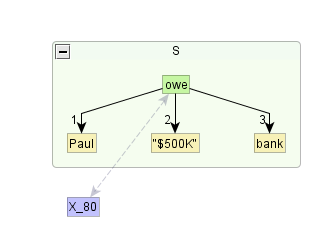
\includegraphics[width=0.6\textwidth, trim = {0cm 0cm 0cm 0cm},clip]{ch3/figs/inspecteur_root.png}
	\vspace{-0.5cm}
	\caption{application de root\_standard}
	\label{fig:rootstand}
\end{figure}

\subsubsection{lex standard : owe (satisfait les contraintes du noeud)}
Par la suite, la règle de lexicalisation standard s'applique. Cela est possible parce que le système regarde dans le semanticon pour l'unité sémantique dans le graphe d'input. Si elle existe dans le semanticon, alors il regarde ce qu'il y a à l'intérieur. Elle renferme deux lexicalisations possibles : owe et debt. Donc on va tenter ces deux lexèmes pour voir si ça fonctionne. Effectivement le système permet de prendre owe puisque owe est un verbe et qu'il satisfait la contrainte. Mais il permet aussi de prendre debt car celui-ci incorpore des verbes supports qui peuvent satisfaire la contrainte de root. Ainsi, un mécanisme complexe de lexicalisation permettra de prend un noeud sémantique en input et de le scinder en deux lors de l'arborisation. Le verbe support deviendra la racine dans ce cas. et le mot debt deviendra un de ses dépendants. Mais nous n'entreront pas dans les détails. POur cela nous vous renvoyons à Lambrey et Lareau-Lambery. Donc nous constatons qu'à ce point, plusieurs arborisation sont possibles, mais nous choisissons de travailler avec la lexicalisation simple. C'est pourquoi nous optons pour l'arborisation qui prend le verbe owe comme racine. 
\begin{figure}[htb]
	\centering
	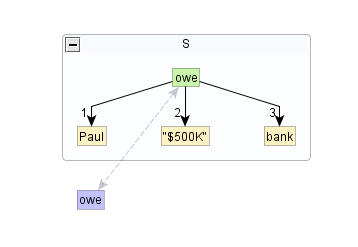
\includegraphics[width=0.7\textwidth, trim = {0cm 0cm 0cm 0cm},clip]{ch3/figs/lex_standard_root.png}
		\vspace{-0.5cm}
	\caption{application de lex\_standard}
	\label{fig:lexstand1}
\end{figure}

\subsubsection{actant gp : crée les branches et les noeuds vides}
Une fois que owe est lexicalisé, cela déclenche l'application de la règle actant\_gp. Pour chaque relation actancielle, elle puise dans le patron de régime de l'entrée lexicale quelconque. Puis elle fait la conversion des actants sémantiques en actants syntaxiques. OWe a trois actants sémantiques dans l'input. Ils seront réalisés en actants syntaxiques en fonction de la diathèse de cette entrée. (parler de la diathèse). Le patron de régime\draft{utiliser la macro pour gp} de owe impose des restrictions aux actants syntaxiques. La partie de discours doit être X. Au bout de ces branches nouvellement ajoutées, on crée des noeuds vides, mais contraints par une partie du discours spécifique.
\begin{figure}[htb]
	\centering
	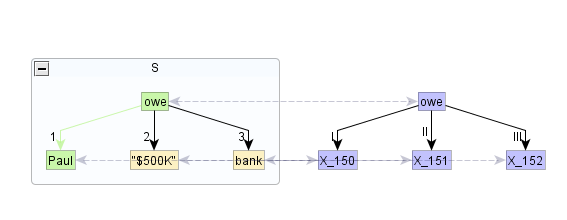
\includegraphics[width=1\textwidth, trim = {0cm 0cm 0cm 0cm},clip]{ch3/figs/actant_gp1.png}
	\caption{application de actant\_gp}
	\label{fig:actantgp}
\end{figure}

\subsubsection{lex class et lex standard}
Donc, la suite des choses est de répétée la phase de lexicalisation puisque nous avons des noeuds non-étiquetés. Alors on regarde l'unité sémantique spécifiée dans l'input qui est 'bank' 'paul' '\$500'. On va donc regarder dans le semanticon s'ils s'y trouvent. On trouvera 'bank' et sa lexicalisation 'bank' mais pas 'Paul' ni '\$500' car ceux-ci ont le trait 'class' en input. Donc lex\_standard s'applique et on lexicalise 'bank' au noeud du IIIe\draft{comment mettre le petit e} actant syntaxique car il satisfait les contraintes du noeud. Effectivement, dans le lexicon 'bank' est de type dpos=N ce qui correspond à la contrainte demandée par la règle actant\_gp précédement via le gp du verbe owe. Pour ce qui est de 'Paul' et '\$500', ils ont le trait class dans l'input sémantique. C'est là que la règle de lex\_class entre en ligne de compte. Elle passer directement au lexicon, puisque les sens ne sont pas encodés dans le semanticon comme les classes ont des comportements prédictibles. Dans le lexicon par contre, c'est là que les classes sont décrites. Effectivement la classe proper\_noun et la classe numeral vont permettre l'application de la règle lex\_class et de lexicaliser paul et 500 piastres. Les classes ont les informations de type dpos et autres traits grammaticaux. L'étiquette du noeud sémantique est directement copiée en syntaxe. on s'assure finalement que les contraintes de ces classes respectent les contraintes du noeuds généré par gp\_actant. Lorsque c'est le cas, la lexicalisation se produit. Les noms propres héritent des traits de la classe des noms, donc la dpos est là, puis les montants héritent des traits de la classe des nombres.

\begin{figure}[htb]
	\centering
	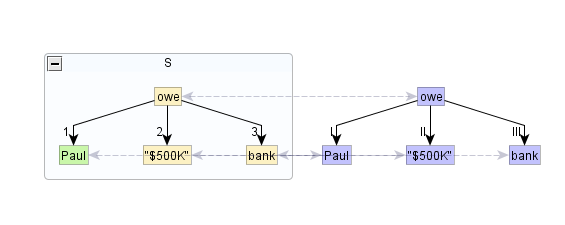
\includegraphics[width=1\textwidth, trim = {0cm 0cm 0cm 0cm},clip]{ch3/figs/lex_standard2.png}
	\caption{application de lex\_standard}
	\label{fig:lexstand2}
\end{figure}

\subsubsection{traits grammaticaux}
\draft{à revoir, pourquoi j'avais ajouté ça dans mon plan}


\subsection{2ème phase: RSyntP à RSyntS}

\subsubsection{lex class et lex lu}
On va chercher les lexicalisations de surface de chacune des unités lexicales. Provenant des classes et des entrées directement. \draft{demander à françois à quoi sert cette étape}. Lex class fait paul et 500 , puis lex lu fait bank et owe.
\begin{figure}[htb]
	\centering
	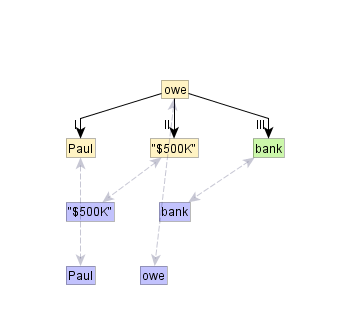
\includegraphics[width=0.7\textwidth, trim = {0cm 0cm 0cm 0cm},clip]{ch3/figs/rsyntslexicalisation1.png}
	\caption{application de lex class et lex lu}
	\label{fig:lexsurf}
\end{figure}

\subsubsection{synt actant subj}
Réalise la relation subjectale entre le verbe et le nom qui a cette relation. Cette information est encodée dans le gp du verbe owe qui est hérité de verb dit, puis de verb dt jusqu'à verb tout court. Qui dit que son premier actant I, est le sujet.

\draft{peut-être mettre du code inline ici ?}

\subsubsection{synt actant dir}
Crée la relation d'objet direct entre le verbe et l'actant II. Cela est encodé via le verbe owe, qui est un verbe dit, donc hérité de verb dt, qui a comme info que son IIe actant correspond à la relation objet direct.

\subsubsection{synt actant prep}
Celle-ci est la plus complexe des règles actancielles de surface. Car elle va prendre un noeud syntaxique profond et le scinder en 2 pour réaliser le mot fonctionnel qu'est la préposition. 

\subsubsection{det def}
Cette règle de surface ajoute les déterminants.

La figure \ref{syntsurf} démontre l'application simultanée de toutes ces règles de surface.

\begin{figure}[htb]
	\centering
	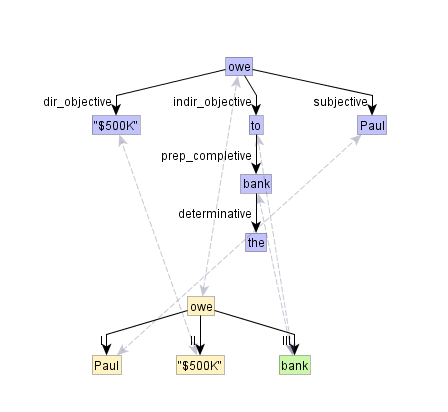
\includegraphics[width=0.7\textwidth, trim = {0cm 0cm 0cm 0cm},clip]{ch3/figs/rsynts_syntactisation.png}
	\caption{application de subj,dir et prep}
	\label{fig:syntsurf}
\end{figure}

%%%%%%%%%%%%%%%%%%%%%%%%%%%%%%%%%%%%%%%%%%%%%%%%
% --------- P R O B L É M A T I Q U E ---------
%%%%%%%%%%%%%%%%%%%%%%%%%%%%%%%%%%%%%%%%%%%%%%%%

\section{Problématique}\label{problema}
La raison d'être de ce mémoire prend vie à cause de GenDR. En travaillant avec ce réalisateur profond pour réaliser divers types d'output et en voulant couvrir le plus large possible les phénomènes langagiers, on s'est rendu compte que la couverture d'un réalisateur passe impérativement par les verbes. Ainsi, pour avoir une meilleure couverture des verbes, nous nous sommes retournés vers les dictionnaires de verbes. Plus précisément des dictionnaires contenant de l'information de nature lexicale sur les verbes. Si on a accès aux patrons de régime d'une grande quantité de verbe, notre couverture se vera largement agrandie.Ça c'est la première raison, plus théorique et pragmatique. 

D'ailleurs, 

présenter les limites de ce système et pourquoi nous voulions aller chercher l'aide d'une ressource comme VerbNet pour pallier à ce problème.
mentionner les dictionnaires qui disent que les verbes sont les plus importants
Expliquer c'est quoi un patron de régime/cadre de sous-catégorisation, valence, etc.
permettent de couvrir large
patrons de régime des verbes y sont encodés
\draft{est-ce que je parle de ce problème ici, ou pas du tout, ou bien juste quand on parle du gpcon directement: problématique liée aux verbes : mécanisme d'héritage pas capable d'avoir deux parties du discours différentes pour un objet direct par exemple, restreint le nombre de génération, ou ça peuple inutilement le dictionnaire d'entrée verbale par type de complément qu'il prend. Pas logique en aucune manière. C'est là qu'un dictionnaire de patron de régime entre en ligne de compte}.
Forge utilise un dictionnaire de valence, aussi un héritié de MARQUIS utilise un dictionnnaire de valence.